\section{План изменения архитектуры}

План изменения архитектуры должен представлять собой 
последовательные шаги для внедрения новой архитектуры в старую систему.

Важно понимать, что сложно внедрить всю архитектуру целиком, и лучше использовать для этого отдельные шаги.

Помимо этого, отдельные шаги позволяют так же протестировать различные системы и приобрести уверенность, 
что итоговая реализация архитектура будет корректно работать и успешно справляться с необходимыми нагрузками.

План переноса архитектуры можно разделить на четыре основные части:

\begin{itemize}
    \item Разворачивание основных систем.
    \item Перенос данных в новые схемы и хранилища.
    \item Пошаговая замена и встраивание различных сервисов в текущую систему.
    \item Полный переход на новую архитектуру.
\end{itemize}

\subsection{Разворачивание основных систем}

Предварительно необходимо развернуть необходимые системы, такие как:

\begin{itemize}
    \item СУБД MongoDB для хранения исходных кодов пользователя и протоколов тестирования.
    \item СУБД Redis для хранения кэшей и в качестве бэкенда для воркеров ejudge-listener и Rmatics.
    \item Rmatics в качестве основной системы;
    \item ejudge-listener для обновления статусов посылок и сбора протоколов;
\end{itemize}

Для начала необходимо определиться, 
на каких виртуальных машинах будут развёрнуты системы.
В Информатикс использовались две виртуальные машины, ejudge-vm и moodle-vm (см. рисунок \ref{fig:old_vm}).
Было решено разворачивать сервисы следуя той же логике разбивки сервисов на виртуальные машины, которая была использована до этого: 
все сервисы связанные с пользовательскими интерфейсами (Rmatics и rmatics-workers), 
а так же СУБД (СУБД Redis и СУБД MongoDB) было решено развернуть на виртуальной машине moodle-vm,
а сервисы, связанные с Ejudge (ejudge-listener и ejudge-listener-workers),
было решено развернуть на виртуальной машине ejudge-vm.

Схему соотношения сервисов и виртуальных машин можно посмотреть на рисунке \ref{fig:new_vm}.

\begin{figure}
  \centering
  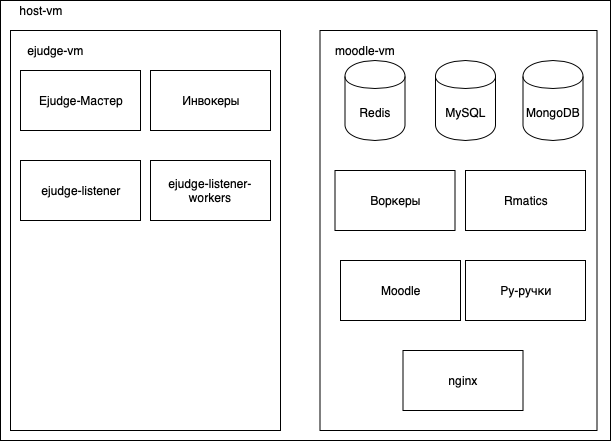
\includegraphics[width=\textwidth]{figures/new_vm.png}
  \caption{Новая схема виртуальных машин Информатикс}
  \label{fig:new_vm}
\end{figure}


Для разворачивания СУБД MongoDB в CentOS достаточно добавить официальный репозиторий MongoDB и установить необходимый пакет через стандартный менеджер пакетов yum.

Однако опытным путём было выяснено, что стандартный конфигурационный файл
обладал существенным недостатком: он не ограничивал количество потребляемой кэшом СУБД оперативной памяти (оперативное запоминающее устройство, ОЗУ).
Данный недостаток был исправлен добавлением в конфигурационный файл максимального количества потребляемой кэшами СУБД.

MongoDB будет запускаться и управляться стандартным для CentOS способом,
с помощью системы systemd.
Конфигурационный файл systemd (юнит) был автоматически добавлен при установке.

Для разворачивания СУБД Redis нужно установить пакет Extra Packages for Enterprise Linux (EPEL) \cite{redis_install}.
Затем можно будет установить СУБД Redis через стандартный менеджер пакетов yum.

Redis будет запускаться и управляться стандартным для CentOS способом,
с помощью системы systemd.
Конфигурационный файл systemd (юнит) был автоматически добавлен при установке.

Установка реализованных сервисов, таких как ejudge-listener и Rmatics потребудет больше усилий.

Оба сервиса написаны на Python и требуют установки различных Python-пакетов для корректной работы.
Для установки различных окружений был использован стандартный для Python менеджер пакетов -- pip и утилита для управлений окружениями Python virtualenv. Оба сервиса будут работать под управлением стандартной для CentOS системы systemd.

Для удобной установки и дальнейшего обновления сервисов были написаны конфигурационные файлы (роли) с помощью использования технологии Ansible.

Ansible -- система управления конфигурациями, написанная на Python, с использованием декларативного языка разметки для описания конфигураций.
Используется для автоматизации настройки и развертывания программного обеспечения. 
Обычно используется для управления Linux-узлами, но Windows также поддерживается. 
Поддерживает работу с сетевыми устройствами, на которых установлен Python версии 2.4 и выше по SSH или WinRM соединению.

Ansible-роли совершают следующие действия для установки сервисов на целевых серверах:

\begin{itemize}
    \item архивируют исходный код;
    \item доставляют исходный код на сервер;
    \item создают необходимые Python-окружения при помощи virtualenv;
    \item перемещают исходный код в необходимые директории;
    \item при необходимости обновляют необходимые systemd-юниты;
    \item запускают или перезапускают сервисы.
\end{itemize}

\subsection{Перенос данных в новые системы и хранилища}

\label{chap:move_data}
Для того, чтобы новая система начала функционировать,
необходимо было осуществить перенос данных из текущих хранилищ в новые.

Нужно скопировать информацию о посылках из текущих таблиц в таблицу pynfotmatics.runs. 
Также нужно перенести данные с файловой системы в СУБД MongoDB.

Для того, чтобы скопировать информацию о посылках из текущих таблиц, 
был написан скрипт на языке SQL, копирующий данные в pynformatics.runs.

Чтобы не нагружать Информатикс, был создан бэкап СУБД MySQL,
который затем был развёрнут на другом сервере. 
Был запущен SQL-скрипт, и таблица pynformatics.runs наполнилась необходимыми данными.
После этого был создан бэкап отдельной таблицы, pynformatics.runs.
Этот бэкап был перенесён на основной сервер Информатикс, а затем был запущен механизм восстановления данных в нужную таблицу.

Таким образом было перенесено более 15 миллионов посылок.
Однако стоит учесть, что посылки, которые появлялись начиная со времени бэкапа СУБД MySQL из Информатикс и до введения отправки посылок через Rmatics,
в pynformatics.runs не перенесены, и был написан отдельный SQL-скрипт,
добавляющий в pynformatics.runs только недостающие посылки.

Для того, чтобы перенести данные о результатах тестирования и исходных кодах пользователя, 
были предприняты аналогичные действия.

Чтобы не нагружать сайт, бэкап посылок и протоколов был развёрнут на другом сервере.
Был написан скрипт на Python, собирающий протоколы и исходный код, 
и сохраняющий данные в MongoDB. 

После этого СУБД MongoDB на этом сервере была остановлена, 
а блобы базы данных были перенесены на сервер Информатикс.
Затем эти блобы были перенесены в директорию данными MongoDB.

Таким образом было перенесено более 15 миллионов исходных кодов, протоколов и результатов тестирования.
Однако стоит учесть, что данные, которые появлялись начиная со времени бэкапа ФС из Информатикс и до введения отправки посылок через Rmatics,
в MongoDB не перенесены, и был написан отдельный Python-скрипт,
переносящий в MongoDB только недостающие исходные коды, протоколы и результаты тестирования.

\subsection{Пошаговое встраивание сервисов}

Для того, чтобы аккуратно совершить переход на новую архитектуру, 
а так же протестировать различные системы и приобрести уверенность в разработанных решениях, было принято вводить функциональность сервисов постепенно.

Также это дало возможность провести изменение архитектуры таким образом,
чтобы недоступность системы была минимальной.

Был отмечен важный для такого подхода факт факт: 
сервер тестирования Ejudge готов был обработать двукратное увеличение посылок от пользователей.

Как было рассмотрено в главе \ref{chap:move_data}, 
данные после первичного переноса из бэкапов, начали рассинхронизироваться с актуальной информацией о посылках.

Поэтому было принято решение дублировать отправку посылок: 
py-ручки были изменены таким образом, чтобы при отправке посылки в Ejudge,
послыка также отправлялась бы и в Rmatics.
Rmatics затем так же пересылал эту посылку в Ejudge, 
Очевидно, что идентичные посылки одинаково тестировались и имели одинаковый результат и протокол тестирования. Исходник посылки оказывался в MongoDB,
а данные о посылке -- в СУБД MySQL в таблице pynformatics.runs.
Это дало возможность сразу решить проблему рассинхронизации пользователей.

Затем py-ручки были изменены таким образом, 
чтобы запрос списка посылок пользователя по задаче, 
списки посылок по пользователям и списки посылок по задача, а так же запроос на изменнеие статуса посылки, не обрабатывался самими py-ручками,
а перенаправлялся в сервис Rmatics.
Также в Rmatics были перенаправлены запросы на просмотр исходников,
запросы на выдачу результатов и протоколов тестирования.

Это дало возможность проверить, что отправка посылок,
обновление статусов и выбор списка посылок пользователей обрабатываются корректно.
На этом этапе пользователи видели посылки, результаты тестирования и протоколы, 
работающие через новую систему,
однако данные мониторов всё ещё собирались через старую систему.

Это привело к следующим казусам: при изменении посылки через пользовательский интерфейс, мог поменяться и монитор.
Однако теперь при запросе изменения посылки из интерфейса менялись посылки в таблице pynformatics.runs, а не в старой системе.
Таким образом, пользователи меняли статусы посылок, но соответствующие мониторы не менялись.

Следующим этапом стало введение в работу новых систем сбора данных для мониторов.
Раньше мониторы собирались внутри PHP-кода.
Для того, чтобы переложить эту логику на Rmatics, в py-ручках были написано соответствующее API, вызывающее нужное API в Rmatics,
а так же изменён PHP-код таким образом, 
чтобы он не занимался сбором мониторов, 
но только выдавал JavaScript-код, выполняемый в браузере пользователя и обращающийся к соответствующему API py-ручек.

После этого пользователи начали в результатах данные о тестировании,
собирающиеся с использованием систем кэшэй в сервисе Rmatics.

Финальным этапом стало изменение py-ручек таким образом, 
чтобы отключить дублирование посылок.
Теперь все посылки пользователей больше не отправлялись в Ejudge напрямую,
но только через сервис Rmatics.

Таким образом последовательное внедрение новых архитектурных решений в старую архитектуру было завершено.